%\begin{savequote}[75mm]
%Nulla facilisi. In vel sem. Morbi id urna in diam dignissim feugiat. Proin molestie tortor eu velit. Aliquam erat volutpat. Nullam ultrices, diam tempus vulputate egestas, eros pede varius leo.
%\qauthor{Quoteauthor Lastname}
%\end{savequote}

\chapter{The Physics of the Higgs Boson}

This chapter presents an overview of the Standard Model of Particle Physics and in particular the physics of the Higgs boson. First, a brief overview of the Standard Model and its history are presented. Then, a description of the Higgs mechanism of electroweak symmetry breaking is given. Next, the physics of single Higgs boson production and decay is described. The Standard Model also allows for production of two Higgs bosons and this is detailed as well. Finally, di-Higgs production in two beyond the Standard Model (BSM) theories - Randall-Sundrum gravitons (RSG) and Two Higgs Doublet Models (2HDM) - is shown. 

\section{The Standard Model of Particle Physics}

The Standard Model (SM) of Particle Physics is a quantum field theory describing the fundamental particles of nature and the forces that govern their interactions. Several comprehensive treatments of the SM already exist in the literature\cite{Griffiths,HalzenAndMartin,Tully,PDG,Schwartz,Dawson} and this section will not rehash those. Rather, this section presents a brief overview of the SM particles and forces in order to define them for subsequent discussions. 

The Standard Model consists of two primary categories of fundamental particles: fermions (spin $1/2$ particles) and bosons (integer spin particles). The SM also describes three forces: electromagnetism, the weak nuclear force, and the strong nuclear force. Gravity is not included in the theory and is largely irrelevant at the scales currently probed by collider experiments. Within the fermions, there are both quarks (which interact via all three forces) and the leptons. The charged leptons interact via electromagnetic and weak interactions, while neutrinos (neutral leptons) interact only via the weak force. Within the bosons, there are the $W^{\pm}$ and $Z$ bosons (the mediators of the weak force), the gluon ($g$, the mediator of the strong force), and the photon ($\gamma$), the mediator of the electromagnetic force. Finally, there is the Higgs boson, a fundamental spin-$0$ particle resulting from the Higgs mechanism of electroweak symmetry breaking.  Figure~\ref{fig:sm_particles} summarizes the fermions and bosons of the SM. 

\begin{figure}[h!]
  %\vspace{20pt}
  \centering
  \captionsetup{justification=centering}

  %\hspace*{-32pt}
  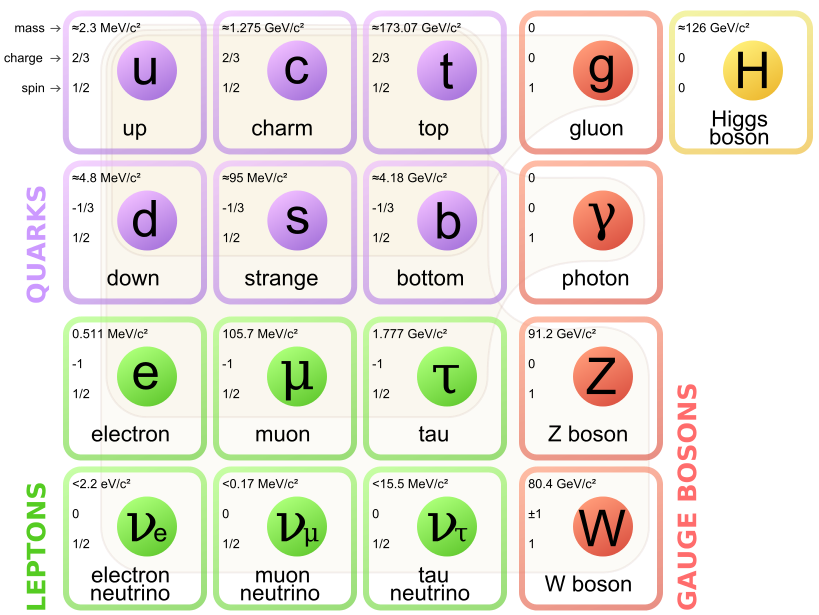
\includegraphics[width=0.6\textwidth]{figures/SM_particles}
  \caption{The particles of the Standard Model and their properties\cite{PDG}.}
  \label{fig:sm_particles}
\end{figure}

The Standard Model coalesced into a unified theoretical framework in the 1960s through the work of Glashow, Weinberg, Salam, and others on the theory of electroweak interactions\cite{Glashow, Weinberg, Salam, Glashow2}. This theory characterized both the electromagnetic and weak interactions as unified under a single gauge symmetry group, namely $SU(2) \times U(1)$. At low enough energy scales (on the order of the $W$ and $Z$ masses, the electroweak symmetry is broken, as evidenced by the fact that the weak bosons have mass while the photon does not. The discovery of the Higgs boson in 2012 confirmed the Higgs mechanism as the most likely candidate for this electroweak symmetry breaking\cite{Discovery, CMSDiscovery}. The electroweak theory is then combined with the theory of quantum chromodynamics (which models the strong sector as a non-abelian $SU(3)$ gauge group) to form the complete SM\cite{QCDBook}. 

\section{Electroweak Symmetry Breaking and the Higgs}

In the Standard Model Lagrangian, it is difficult to include mass terms for the $W$ and $Z$ bosons without breaking the fundamental gauge symmetry of the Lagrangian. A traditional mass term does not preserve the $SU(2) \times U(1)$ symmetry. Additionally, scattering of massive $W$ and $Z$ bosons violate unitarity and these diagrams diverge at high energy scales. In the 1960s, Higgs, Brout, Englert, Guralnik, Kibble, and Hagen developed a mechanism for spontaneous symmetry breaking via the additioanl of a complex scalar doublet to the SM. Three of the four real degrees of freedom of this complex field would go to the longitudinal modes of the $W^{\pm}$ and $Z$, thus allowing them to have mass\cite{Higgs1,Higgs2,Englert,Guralnik}. The remaining degree of freedom would manifest as an additional scalar, known now as the Higgs boson (Higgs was the first to predict the existence of the new particle). 

The mechanism works by introducing a Lagrangian for the newly introduced field that still respects the symmetry of the Standard Model inherently, but with a minimum at a non-zero vaccuum expectation value for the field. In this minimum of the potential, the electroweak symmetry is broken. Specifically, consider a complex scalar doublet $\phiH$ with four degrees of freedom, as shown in equation~\ref{eqn:phi_def}.

\begin{equation}
\label{eqn:phi_def}
\phiH = \left( \begin{array}{c} \phi^+ \\ \phi^0 \end{array} \right) = \frac{1}{\sqrt{2}}\left( \begin{array}{c} \phi_{1}^{+} + i\phi_{2}^+ \\ \phi_1^0 + i\phi_2^0 \end{array} \right)
%\phiH = \left( \begin{array}{c} \phi^+ \\ \phi^0  \end{array}\right) = \left( \begin{array}{c} \phi_1^+ + i\phi_2^+ \\ \phi_1^0 + i \phi_2^0 \end{array}\right) 
\end{equation}

The minimal potential of a self-interacting Higgs that still respects the SM symmetry is given in equation~\ref{eqn:potential}.

\begin{equation}
\label{eqn:potential}
V(\phiH) = \mu^2 \phiH^{\dagger}\phiH + \lambda(\phiH^\dagger\phiH)^2
\end{equation}

If the $\mu^2$ term of this potential is positive, then the potential has a minimum at $\phiH = 0$ and the SM symmetry is preserved. However, if instead $\mu^2 < 0$, then the minimum is at a finite value of $\phiH$, namely

\begin{equation}
\phiH_{\rm min} = \frac{1}{\sqrt{2}} \left(\begin{array}{c} 0 \\ v\end{array} \right)
\end{equation}

where $v = \sqrt{\mu^2/\lambda}$. Because this is the location of the minimum, it corresponds to the vacuum expectation value for the field ($\langle\phiH\rangle = \phiH_{\rm min}$). The excitations of the Higgs can then be parameterized as 

\begin{equation}
\phiH = \frac{1}{\sqrt{2}} \left(\begin{array}{c} 0 \\ v + H \end{array}\right)
\end{equation}

The full scalar Lagrangian, including the kinetic term, is then given as 

\begin{equation}
\mathcal{L}_s = (D^\mu \phiH)^\dagger(D_\mu\phiH) - V(\phiH)
\end{equation}

where the covariant derivative is defined as 

\begin{equation}
D_\mu = \partial_\mu + \frac{ig}{2}\tau^aW_\mu^a + ig'YB_\mu
\end{equation}

and $W^1, W^2, W^3$ and $B$ are the $SU(2)$ and $U(1)$ gauge fields of the electroweak theory, respectively. $g$ and $g'$ are the corresponding coupling constants. With the scalar Lagrangian in place, the physical gauge fields can then be written as 

\begin{equation}
\label{eqn:Weq}
W_\mu^\pm = \frac{1}{\sqrt{2}}(W_\mu^1 \mp iW_\mu^2) 
\end{equation}

\begin{equation}
\label{eqn:Zeq}
Z_\mu = \frac{-g'B_\mu + gW_\mu^3}{\sqrt{g^2 + g'^2}} 
\end{equation}

\begin{equation}
\label{eqn:photoneq}
A_\mu = \frac{gB_\mu + g'W_\mu^3}{\sqrt{g^2 + g'^2}}
\end{equation}

Equation~\ref{eqn:Weq} corresponds to the charged $W^+$ and $W^-$ bosons, equation~\ref{eqn:Zeq} corresponds to the neutral $Z$ boson, and equation~\ref{eqn:photoneq} corresponds to the neutral photon. The masses of the particles also arise from the Lagrangian. The photon has zero mass, while the masses of the $W$ and $Z$ bosons are given in equation~\ref{eqn:bosonmasses}.

\begin{equation}
\label{eqn:bosonmasses}
\begin{array}{c}
M_W^2 = \frac{1}{4}g^2v^2 \\ 
M_Z^2 = \frac{1}{4}(g^2 + g'^2)v^2
\end{array}
\end{equation}

The fermion masses also arise through a coupling with the Higgs via the Yukawa interaction (for a detailed description, see\cite{Dawson}). In this case the coupling between the Higgs and the fermions goes as 

\begin{equation}
\label{eqn:higgs-fermions}
g_{Hf\bar{f}} = \frac{m_f}{v}
\end{equation} 

The full Lagrangian of Higgs interactions can be written as 

\begin{equation}
\mathcal{L}_{\rm Higgs} = -g_{Hf\bar{f}}\bar{f}fH + \frac{g_{HHH}}{6}H^3 + \frac{g_{HHHH}}{24}H^4 + \delta_V V_\mu V^\mu\left(g_{HVV} H + \frac{g_{HHVV}}{2}H^2\right)
\end{equation}

with 

\begin{equation}
\begin{array}{cc}
g_{HVV} = \frac{2m_V^2}{v} & g_{HHVV} = \frac{2m_V^2}{v^2} \\ 
g_{HHH} = \frac{3m_H^2}{v} & g_{HHHH} = \frac{3m_H^2}{v^2}
\end{array}
\end{equation}

Here, $V$ refers to the $W^{\pm}$ and $Z$, and $\delta_{W} = 1$ while $\delta_Z = 1/2$. Phenomenologically, there are a few features of this Lagrangian that are useful to note. First, note that the Higgs mass is a free parameter of the theory that must be determined experimentally. Second, note that the coupling of the Higgs to the vector bosons and fermions scales with the masses of these particles, a fact that is important when considering both the production and decays of the particle. Also note that the branching ratio of the Higgs to $W$ bosons will be twice that of the branching ratio to $Z$ if the Higgs mass is large enough to produce the particles on shell because of the extra symmetry factor associated with the $W$ coupling. Finally, note the presence of the cubic and quartic Higgs self interaction terms, which can lead to final states with multiple Higgs bosons produced. 

\section{Higgs Boson Production and Decay}

This section discusses the properties of Higgs production and decay mechanisms. The details presented here will focus on the properties of a $125 \GeV$ Higgs boson, as this is the mass closest to that of the newly discovered Higgs. 

\subsection{Higgs production}

The Higgs is produced by four main production modes at the Large Hadron Collider - gluon-gluon fusion (ggF), vector boson fusion (VBF), associated production with a $W$ or $Z$ boson, or associated production with top quarks ($\ttbar H$). Figure~\ref{fig:production_modes} shows the Feynman diagrams for these four modes. 

\begin{figure}[h!]
  %\vspace{20pt}
  \centering
  \captionsetup{justification=centering}

   \begin{subfigure}[t]{0.5\textwidth}
        \centering
        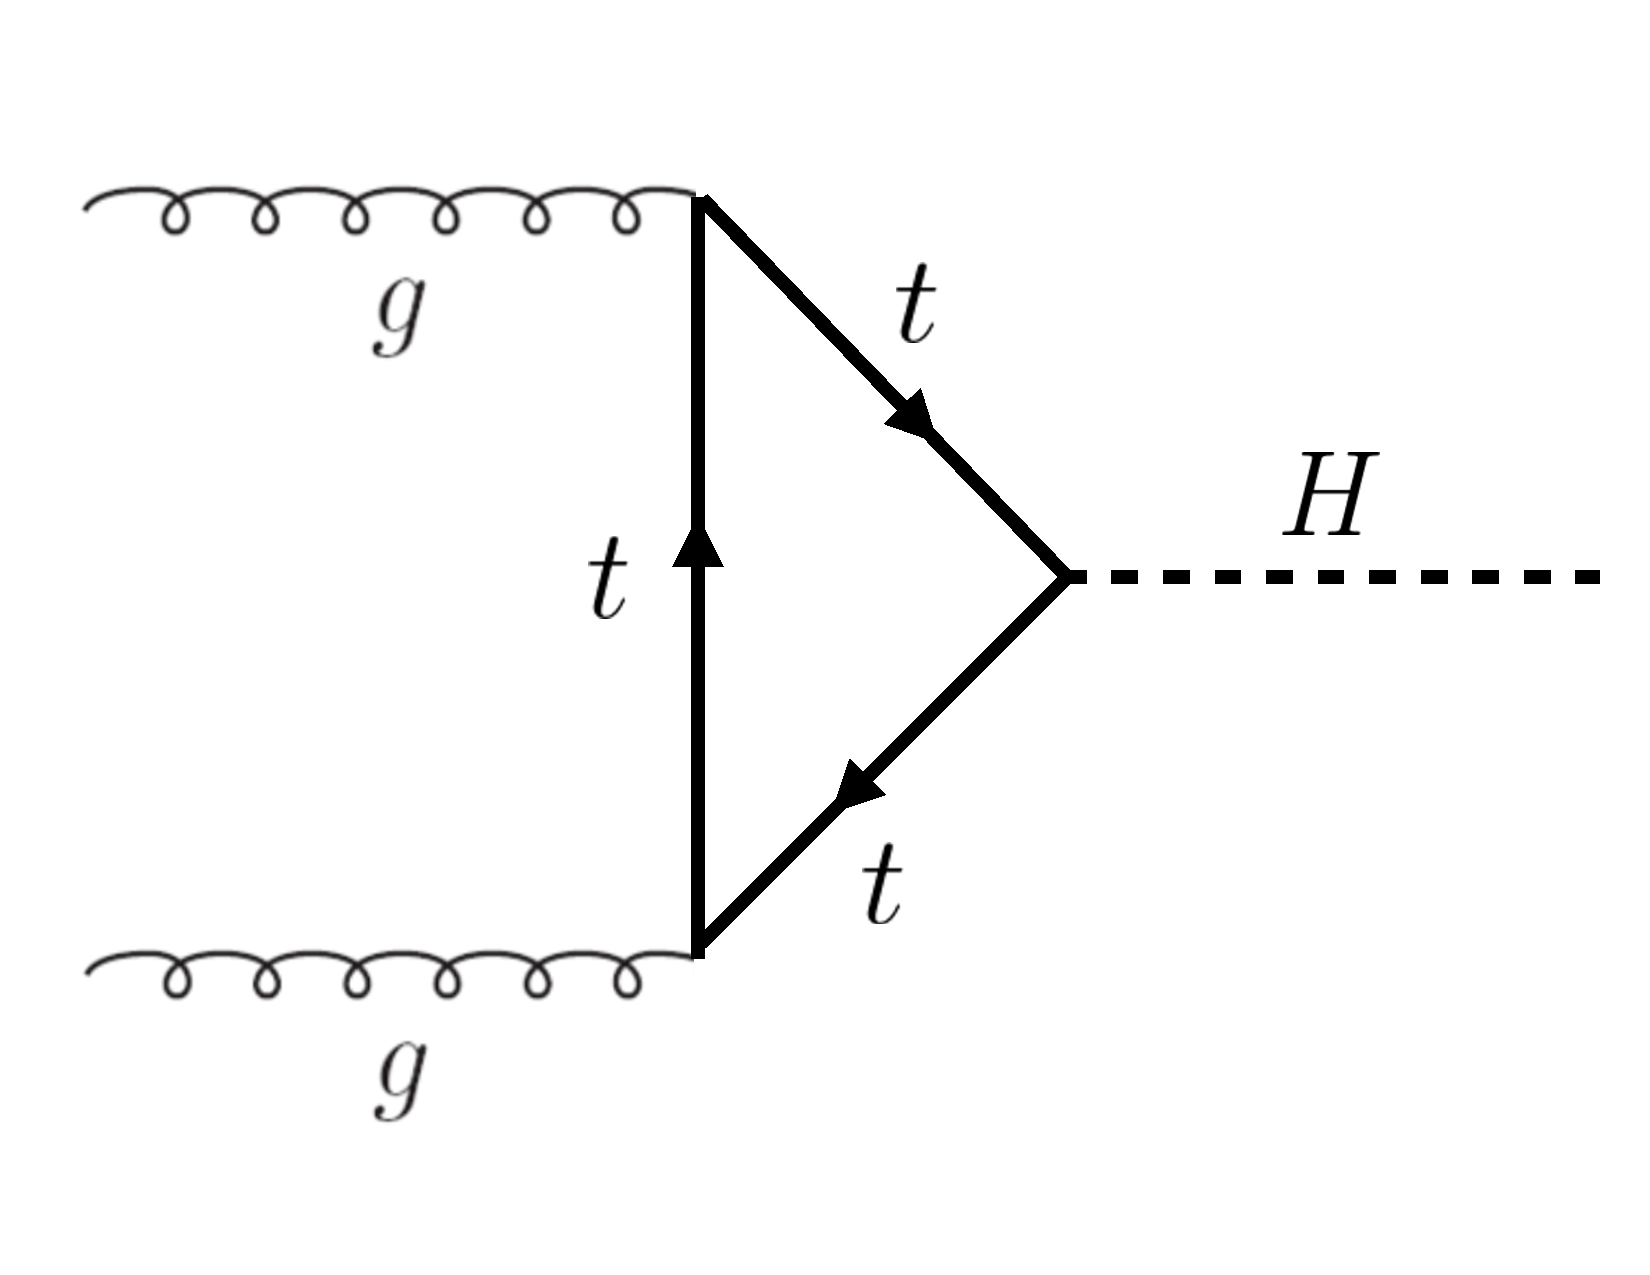
\includegraphics[width=0.6\textwidth]{figures/ggF_Higgs}
        \caption{}
    \end{subfigure}%
    \begin{subfigure}[t]{0.5\textwidth}
        \centering
        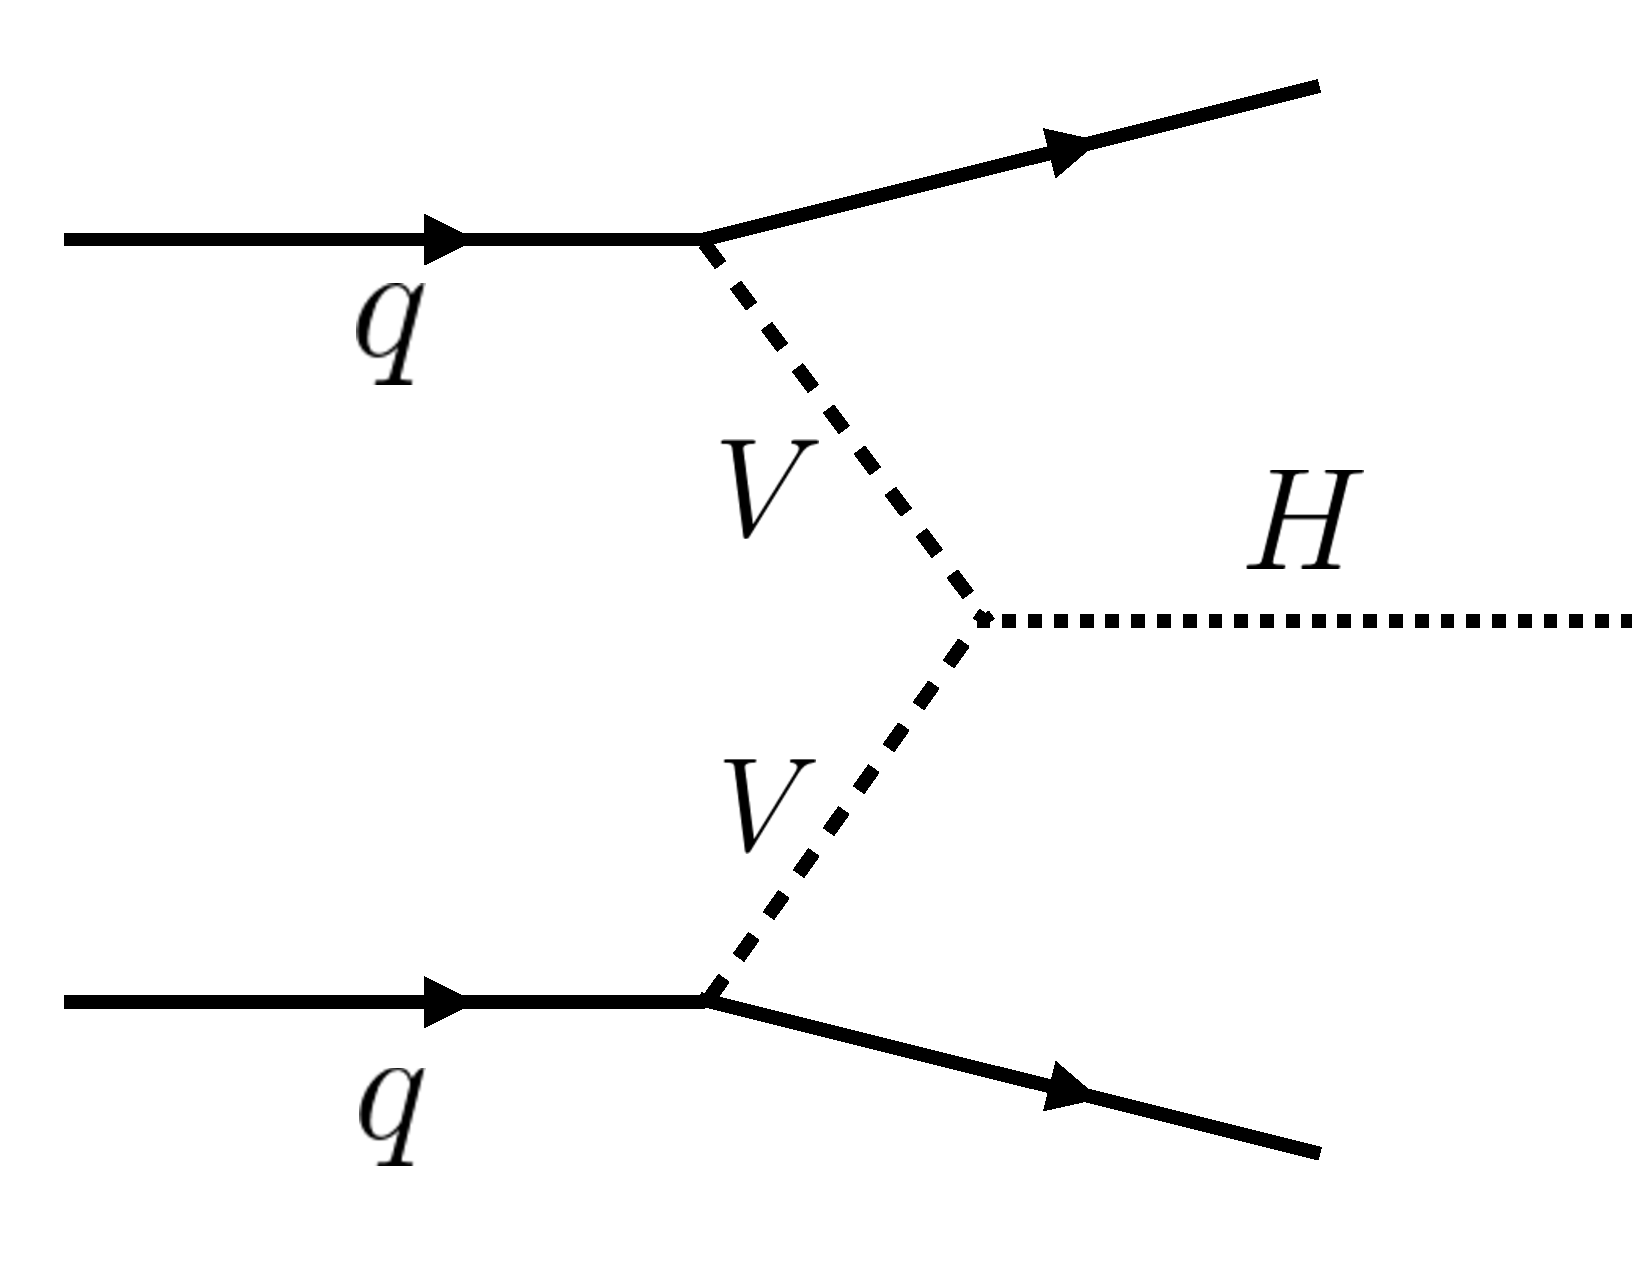
\includegraphics[width=0.6\textwidth]{figures/VBF_Higgs}
        \caption{}
    \end{subfigure}

    \begin{subfigure}[t]{0.5\textwidth}
        \centering
        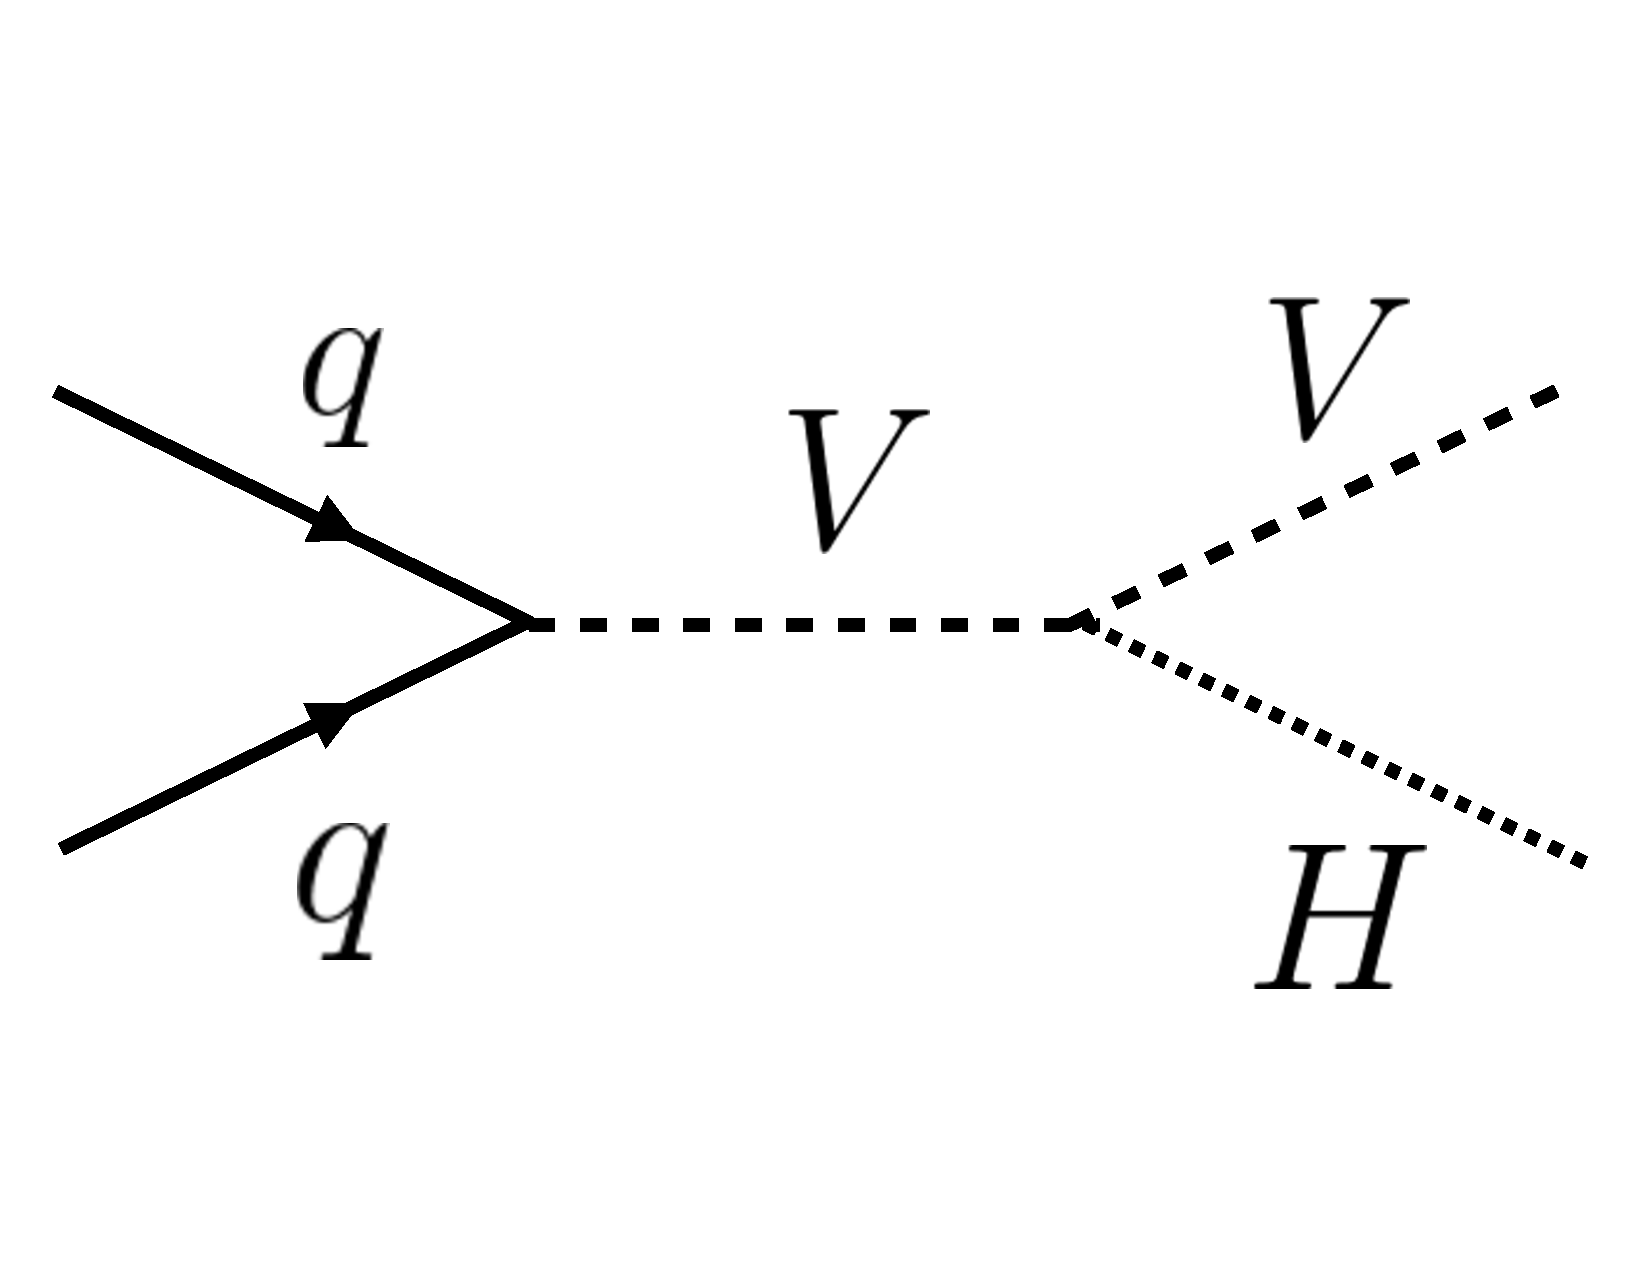
\includegraphics[width=0.6\textwidth]{figures/V_higgs}
        \caption{}
    \end{subfigure}%
    \begin{subfigure}[t]{0.5\textwidth}
        \centering
        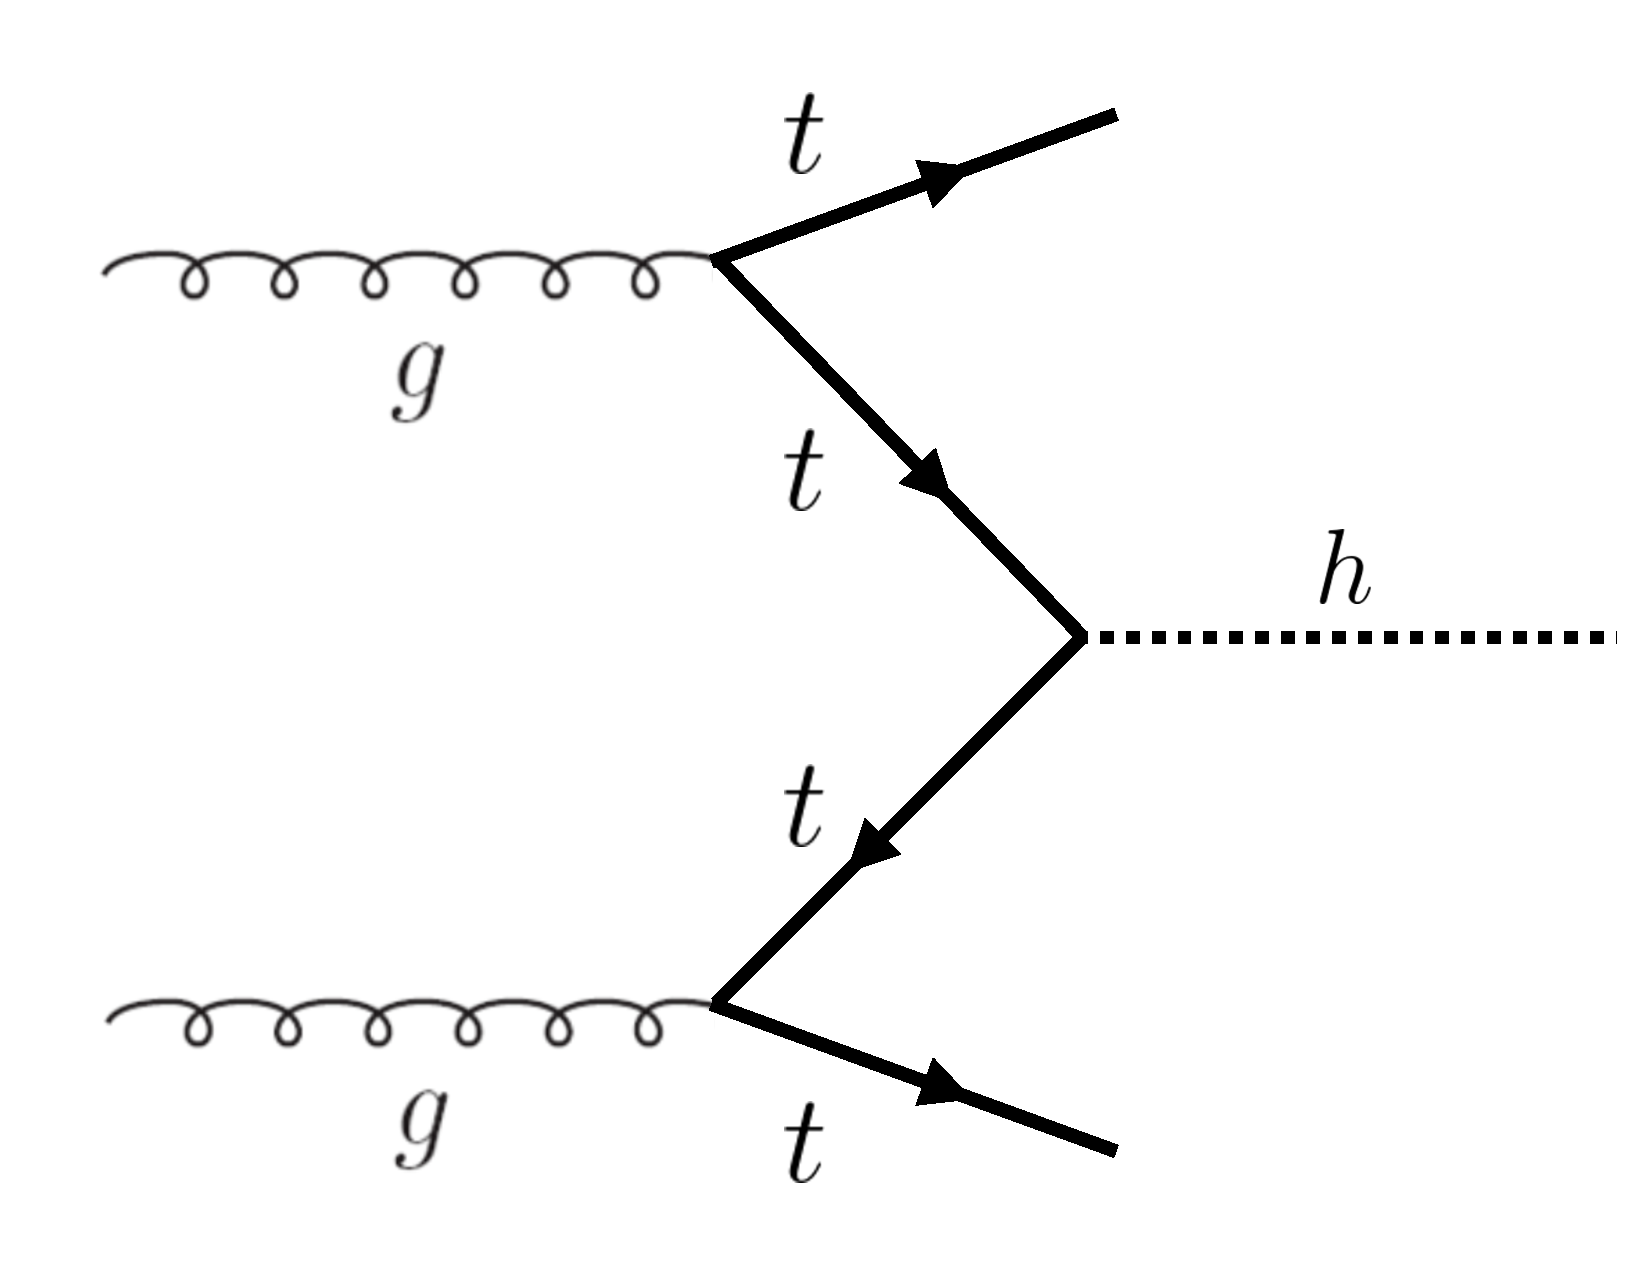
\includegraphics[width=0.6\textwidth]{figures/ttH}
        \caption{}
    \end{subfigure}

   \caption{The four most common Higgs boson production modes at the LHC: (a) gluon-gluon fusion, (b) vector boson fusion, (c) $W/Z$ + $H$ production, (d) $\ttbar H$ production}
  \label{fig:production_modes}
\end{figure}

In gluon-gluon fusion, gluons from the incoming protons fuse via a top-quark loop to produce a Higgs. The top quark is the dominant contribution in the loop due to its heavy mass and the fact that the Higgs-fermion coupling constant scales with fermion mass. In vector boson fusion, the incoming quarks each radiate a $W$ or $Z$ boson which fuse to produce the Higgs. This production mode results in a final state with a Higgs boson and two addtional jets which tend to be forward because they carry the longtiduinal momentum of the incoming partons. The Higgs can also be produced in associated with a $W$ or $Z$ boson. The $W/Z$ is produced normally and then radiates a Higgs (this mode is also sometimes known as ``Higgs-strahlung"). Finally, the Higgs can be produced in association with two top quarks. Each incoming gluon splits into a $\ttbar$ pair, and one of the top pairs combines to create a Higgs. 

Figure~\ref{fig:Higgs_xsec} shows the production cross section for a $125 \GeV$ Higgs boson in each of these modes at a $pp$ collider as a function of center of mass energy. 

\begin{figure}[h!]
  %\vspace{20pt}
  \centering
  \captionsetup{justification=centering}

  %\hspace*{-32pt}
  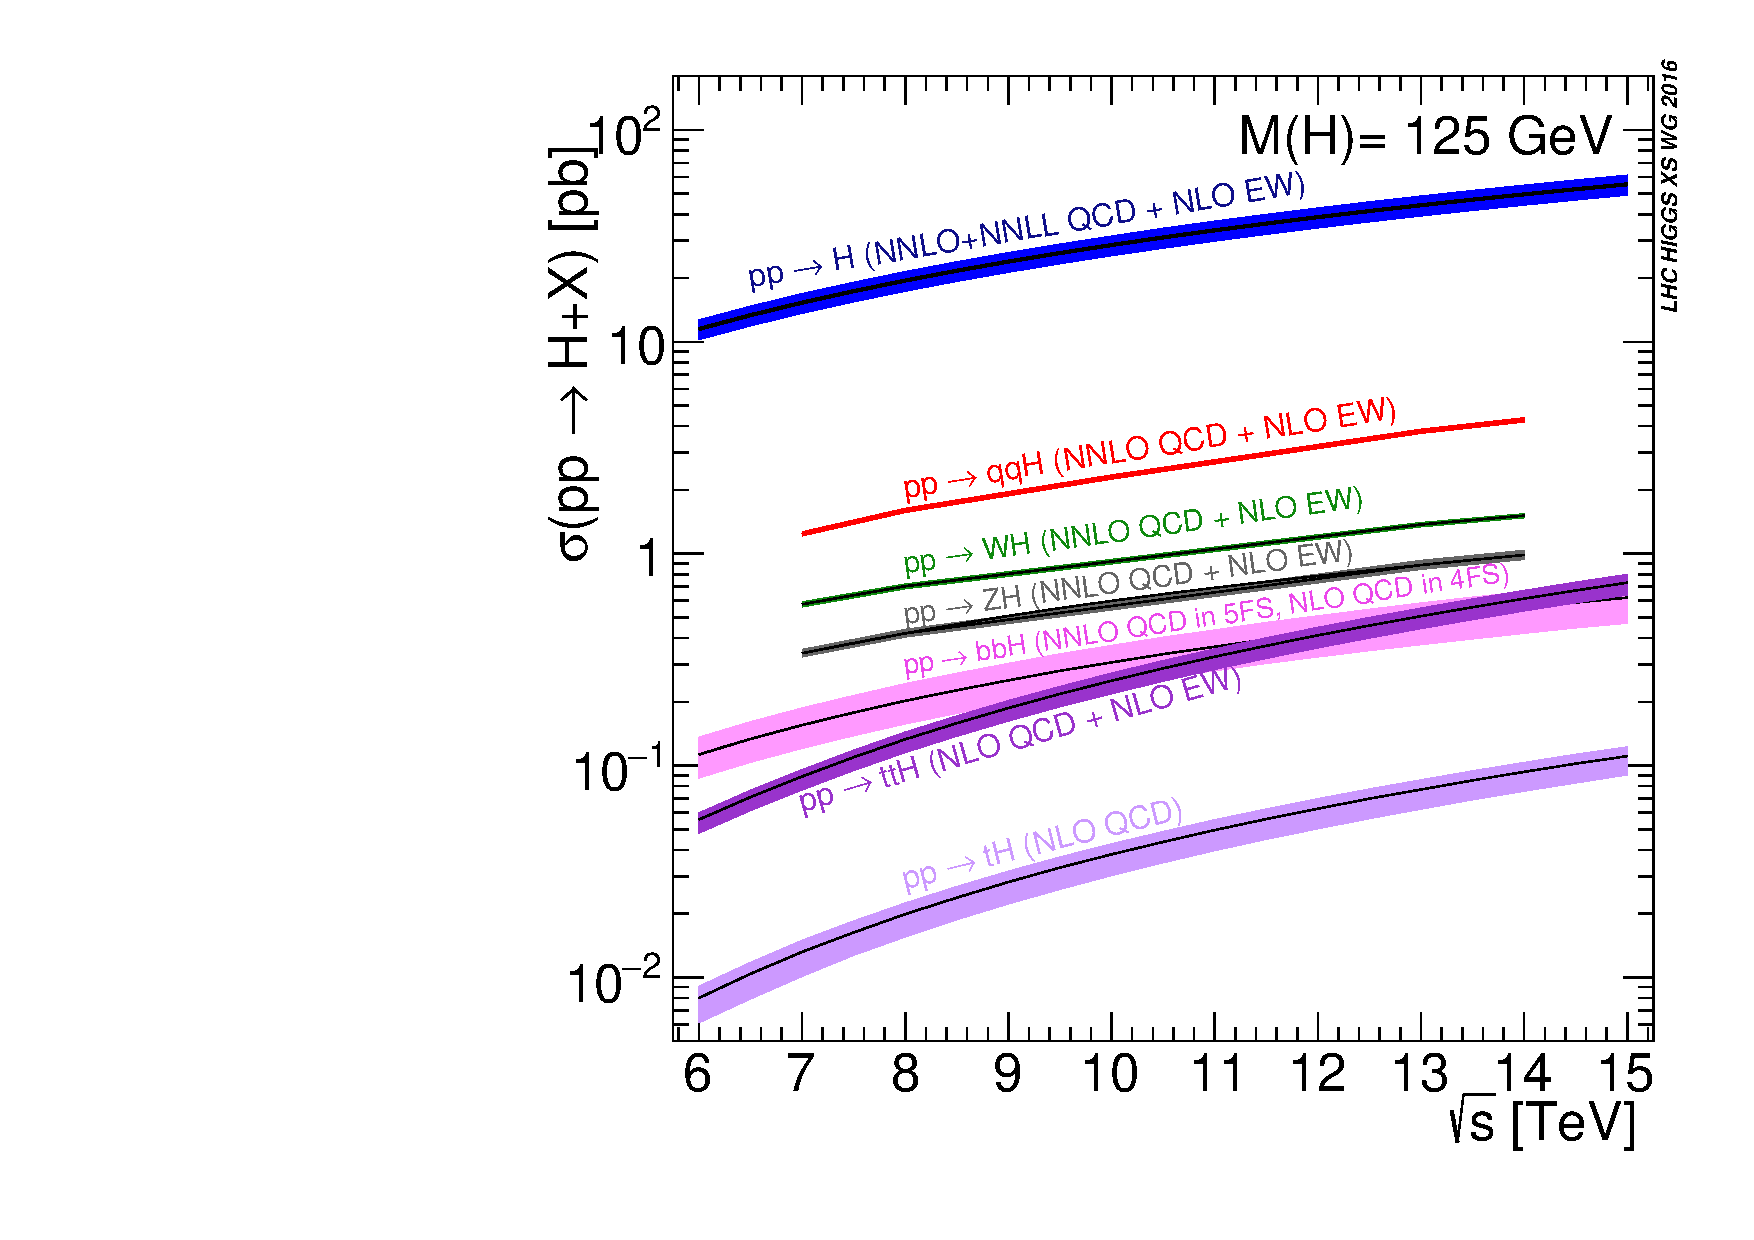
\includegraphics[width=0.6\textwidth,angle=270]{figures/h125_xsec}
  \caption{Higgs production cross sections as a function of center of mass energy ($\sqrt{s}$) at a $pp$ collider\cite{LHCXSWG}.}
  \label{fig:Higgs_xsec}
\end{figure}

In figure~\ref{fig:Higgs_xsec}, note that gluon fusion has the largest cross section, while VBF is the second largest at approximately a factor of $10$ smaller. The figure also includes the less commonly studied $b\bar{b}H$ and $tH$ modes. The $b\bar{b}H$ and $tH$ modes are not studied as commonly as $t\bar{t}H$ due to the larger background contributions and lower cross sections, respectively. At $\sqrt{s} = 8 \TeV$, ggF production of a $125 \GeV$ Higgs has a cross section of $19.47 \pb$, while VBF has a cross section of $1.601 \pb$\cite{LHCXSWG}. The cross sections of all of the main Higgs production modes at this center of mass energy, as well as their uncertainties from varying the renormalization and factorization scales and PDFs, are summarized in table~\ref{tab:Higgs_xsec} for a $125 \GeV$ Higgs.

\begin{table}[h!]
\centering
\captionsetup{justification=centering}
%\begin{tabular*}{0.480\textwidth}{p{0.075\textwidth} p{0.180\textwidth} l}
\hspace{-10pt}
\begin{tabular}{|c|c|c|c|}
\hline
Production mode & $\sigma$ (\pb) & \specialcell{QCD scale \\ uncert. (\%)} & \specialcell{PDF + $\alpha_s$  \\ uncert. (\%)} \\ \hline
Gluon fusion & $19.47$ & $+7.3/-8.0$ & $3.1$ \\ \hline
Vector boson fusion & $1.601$ & $+0.3/-0.2$ & $2.2$ \\ \hline
$WH$ & $0.7026$ & $+0.6/-0.9$ & $2.0$ \\ \hline
$ZH$ & $0.4208$ & $+2.9/-2.4$ & $1.7$ \\ \hline
$t\bar{t} H$ & $0.1330$ & $+4.1/-9.2$ & $4.3$ \\ \hline
$b\bar{b} H$ & $0.2021$ & \multicolumn{2}{c|}{$+20.7/-22.3$} \\ \hline
$tH$ ($t$-channel) & $0.01869$ & $+7.3/-16.5$ & $4.6$ \\ \hline
$tH$ ($s$-channel) & $1.214\times 10^{-3}$ & $+2.8/-2.4$ & $2.8$ \\ \hline
\end{tabular}

\caption{
Production cross sections for a $125 \GeV$ Higgs boson at $\sqrt{s} = 8 \TeV$ with scale and PDF uncertainties~\cite{LHCXSWG}. 
}
\label{tab:Higgs_xsec}
\end{table}



\subsection{Higgs branching ratios}

The fact that the Higgs couples more strongly to more massive particles is crucial for understanding its branching ratios. The width for Higgs decays to fermions is given in equation~\ref{eqn:Hff_width}~\cite{Tully}.

\begin{equation}
\label{eqn:Hff_width}
\Gamma(H\to f\bar{f}) = \frac{N_c \sqrt{2} G_F m_f^2 m_H}{8\pi}
\end{equation}

In this case, $N_c$ is the number of colors, $G_F$ is the Fermi constant, $m_f$ is the mass of the fermion, and $m_H$ is the mass of the Higgs. Note that the width scales with the square of the fermion mass. (This also assumes that the Higgs mass is large enough to decay with both the fermions on shell.) 

The decay width to $WW$ is given in equation~\ref{eqn:HWW_width}~\cite{Tully}. 

\begin{equation}
\label{eqn:HWW_width}
\Gamma(H\to W^+W^-) = \frac{\sqrt{2} G_F M_W^2 m_H}{16\pi}\frac{\sqrt{1-x_W}}{x_W}\left(3x_W^2 - 4x_W + 4\right)
\end{equation}

where $m_W$ is the mass of the $W$ and $x_W  = 4M_W^2/m_H^2$. To get the branching ratio to $ZZ$, the equation is divided by $2$ to account for identical particles in the final state, and $x_W$ is replaced with $x_Z = 4M_Z^2/m_H^2$. This is shown in equation~\ref{eqn:HZZ_width}~\cite{Tully}.

\begin{equation}
\label{eqn:HZZ_width}
\Gamma(H\to ZZ) = \frac{\sqrt{2} G_F M_Z^2 m_H}{32\pi}\frac{\sqrt{1-x_Z}}{x_Z}\left(3x_Z^2 - 4x_Z + 4\right)
\end{equation}

These formulas can also be visualized as a function of Higgs mass. Figure~\ref{fig:branching_ratios} shows the branching ratios as a function of the Higgs mass. 

\begin{figure}[h!]
  %\vspace{20pt}
  \centering
  \captionsetup{justification=centering}
  %\hspace*{-32pt}
  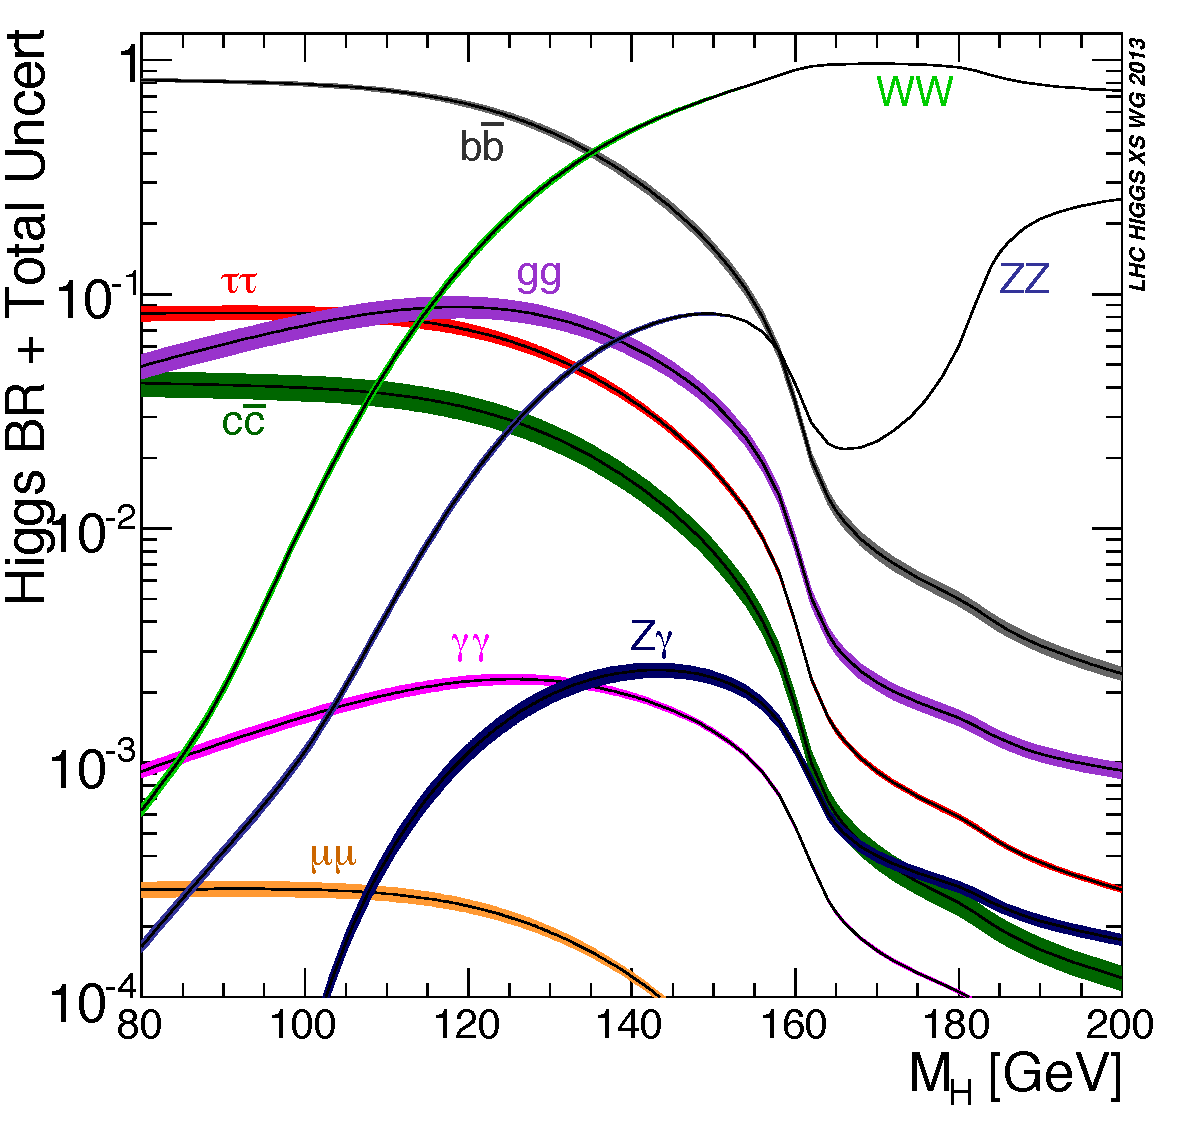
\includegraphics[width=0.6\textwidth]{figures/Higgs_BR}
  \caption{Higgs boson branching ratios as a function of $m_H$\cite{LHCXSWG}.}
  \label{fig:branching_ratios}
\end{figure}

There are a few interesting features to note in this figure. First, note that at high Higgs masses, once on-shell production of both $W$ and $Z$ bosons is possible, these two decays are the dominant ones due to the large masses of the $W/Z$. Also note that the branching ratio to $W$s is twice that of $Z$s at these large masses due to the $\delta_V$ symmetry factor noted previously. At $125 \GeV$, the Higgs is accessible through many different decay modes. The largest branching ratio is the decay $H\to b\bar{b}$ at 58.24\%~\cite{LHCXSWG}. This branching is larger than the $WW$/$ZZ$ decays because one of the two bosons must be produced off-shell for $m_H = 125 \GeV$. The second largest branching ratio is to $WW^*$ at $21.37$ \% (before taking into account the branching ratios of the $W$). Table~\ref{tab:Higgs_BR} summarizes the branching ratios for a $125 \GeV$ Higgs. Note that there is in fact a Higgs branching ratio to $\gamma\gamma$ even though photons are massless. This decay happens through a loop (the largesst contributions to the loop are top and $W$) which suppresses the branching ratio. 

\begin{table}[h!]
\centering
\captionsetup{justification=centering}

%\begin{tabular*}{0.480\textwidth}{p{0.075\textwidth} p{0.180\textwidth} l}
\hspace{-10pt}
\begin{tabular}{|c|c|}
\hline
Decay & Branching ratio (\%) \\ \hline
$b\bar{b}$ & $58.24$ \\ \hline
$WW^*$ & $21.37$ \\ \hline
$gg$ & $8.187$ \\ \hline
$\tau\tau$ & $6.272$ \\ \hline
$c\bar{c}$ & $2.891$ \\ \hline
$ZZ^*$ & $2.619$ \\ \hline
$\gamma\gamma$ & $0.2270$ \\ \hline
$Z\gamma$ & $0.1533$ \\ \hline
$\mu\mu$ & $0.02176$ \\ \hline
\end{tabular}

\caption{
Branching ratios for a $125 \GeV$ Higgs boson\cite{LHCXSWG}. 
}
\label{tab:Higgs_BR}
\end{table}


Note that the branching ratios alone do not tell the full story of which Higgs channels are the most sensitive. For example, a $H\to b\bar{b}$ search in gluon fusion production is incredibly difficult due to the large QCD dijet background at the LHC. However, in associated production of the Higgs, where a $W$ or $Z$ gives additional final state particles that can be used to reduce background, a search for $H\to b\bar{b}$ can be sensitive. The combinations of production and decay modes that are most commonly studied are summarized in table~\ref{tab:sensitive_channels}~\cite{Tully}.

\begin{table}[h!]
\centering
\captionsetup{justification=centering}

%\begin{tabular*}{0.480\textwidth}{p{0.075\textwidth} p{0.180\textwidth} l}
\begin{tabular}{|c|c|c|c|c|}
\hline
Decay & Inclusive (incl. ggF) & VBF & $WH/ZH$ & $t\bar{t}H$ \\ \hline
$H\to\gamma\gamma$ & \checkmark & \checkmark & \checkmark & \checkmark \\ \hline
$H\to b \bar{b}$ & & & \checkmark & \checkmark \\ \hline
$H\to \tau^+\tau^-$ & & \checkmark & & \\ \hline
\HWWfull & \checkmark & \checkmark & \checkmark &  \\ \hline
$H \to ZZ \to 4\ell$ & \checkmark & & & \\ \hline
$H \to Z\gamma \to \ell\ell\gamma$ & very low & & & \\ \hline
\end{tabular}

\caption{
Possible channels for Higgs searches. Checkmarks denote the most sensitive production modes~\cite{Tully}. 
}
\label{tab:sensitive_channels}
\end{table}

\section{Higgs Pair Production in the Standard Model}

The Standard Model also allows for processes that produce two Higgs bosons in the final state, known as Higgs pair production or di-Higgs production. The two main production mechanisms are shown in figure~\ref{fig:diHiggs}.

\begin{figure}[h!]
  %\vspace{20pt}
  \centering
  \captionsetup{justification=centering}

   \begin{subfigure}[t]{0.5\textwidth}
        \centering
        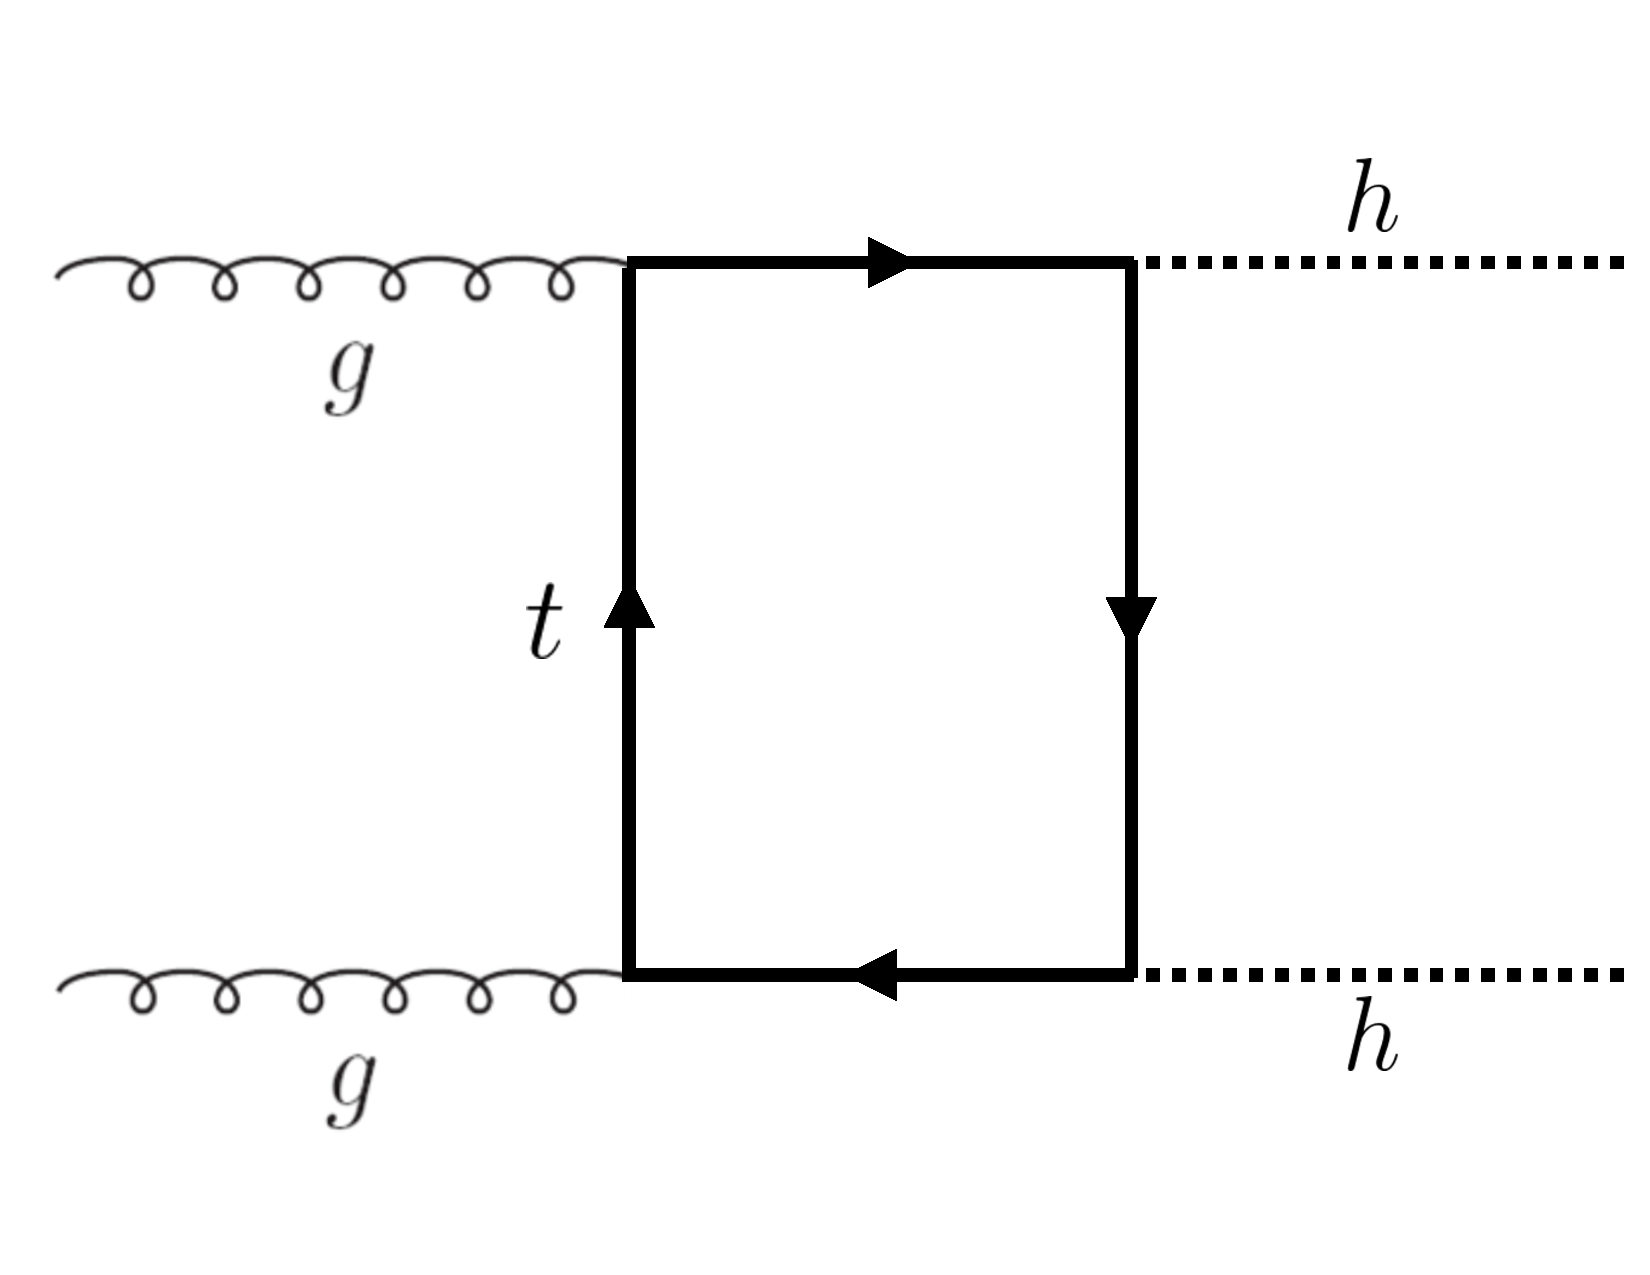
\includegraphics[width=0.7\textwidth]{figures/HH_box}
        \caption{}
    \end{subfigure}%
    \begin{subfigure}[t]{0.5\textwidth}
        \centering
        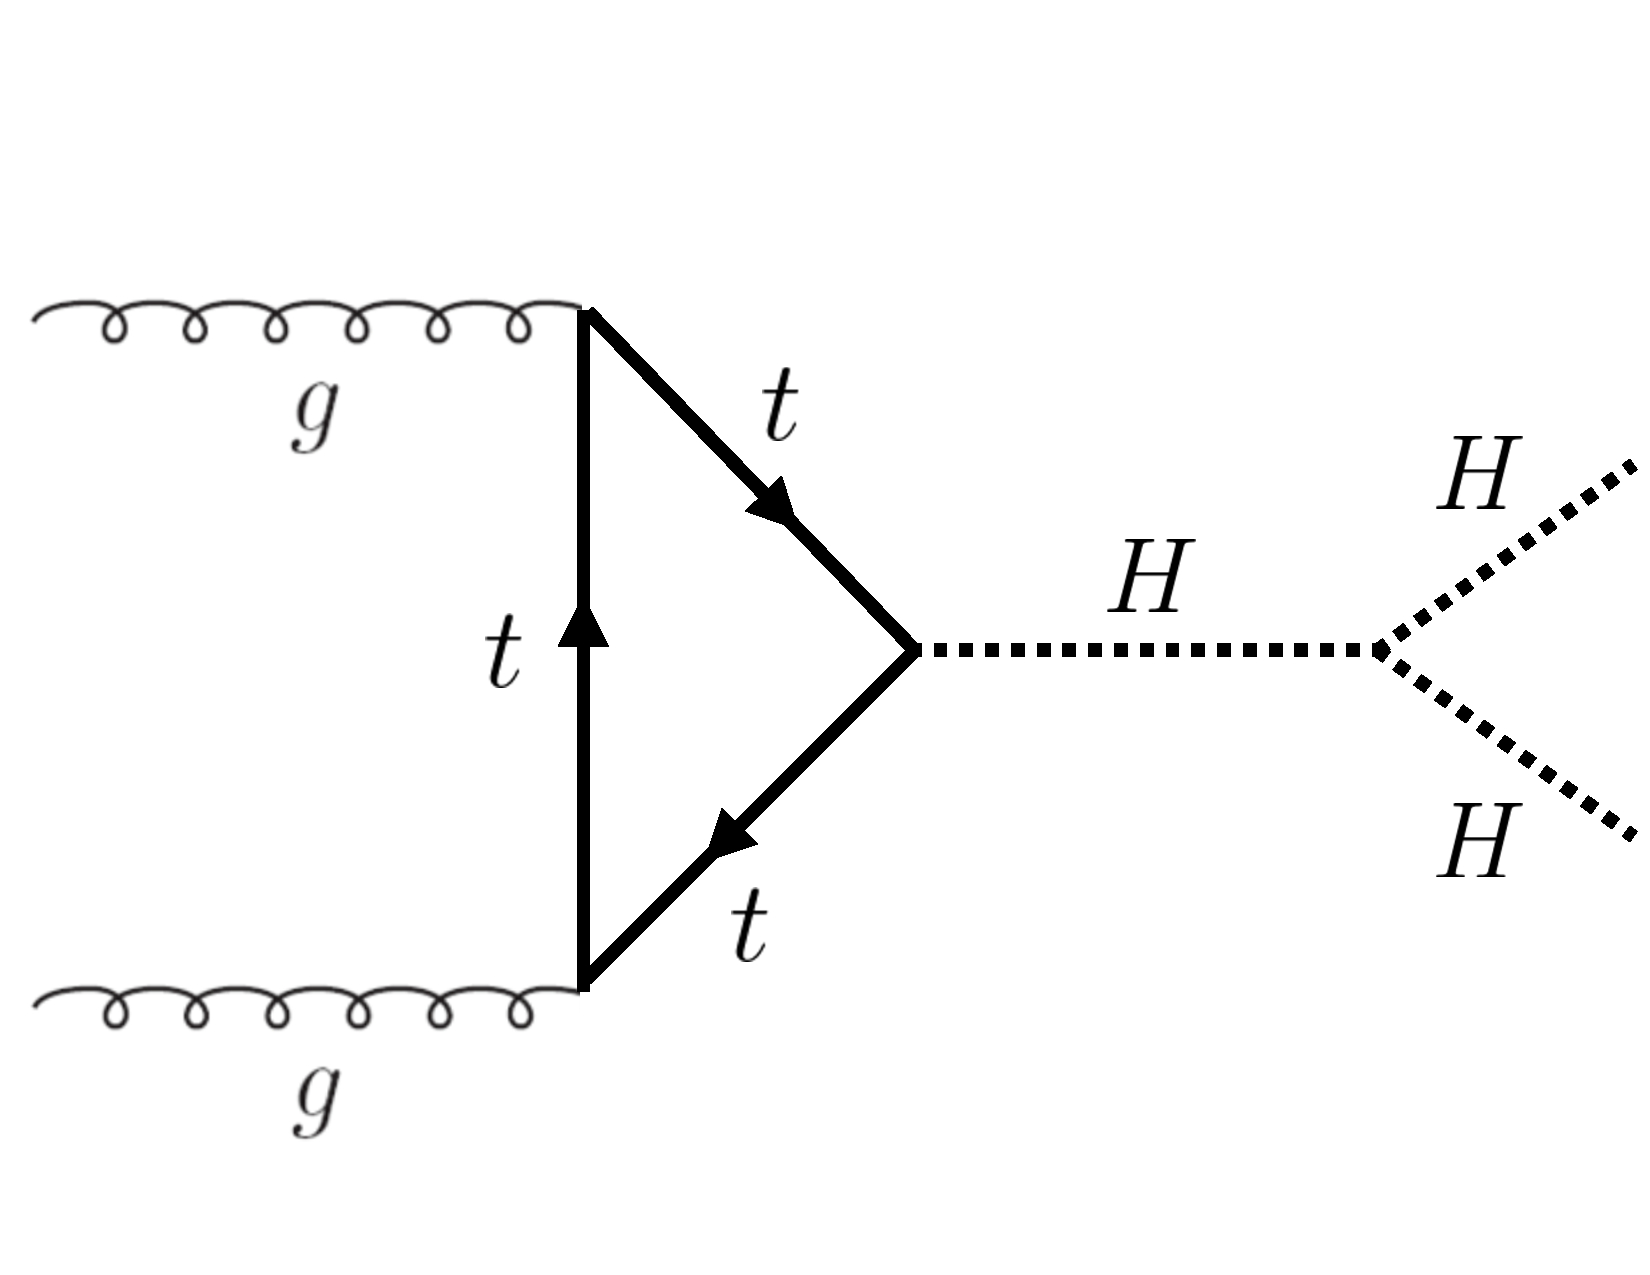
\includegraphics[width=0.7\textwidth]{figures/HH_lambda}
        \caption{}
    \end{subfigure}
   \caption{The two leading diagrams for Standard Model di-Higgs production at the LHC: (a) box diagram, (b) Higgs self coupling}
  \label{fig:diHiggs}
\end{figure}

The two diagrams in figure~\ref{fig:diHiggs} interfere destructively with one another, resulting in a low overall cross section for di-Higgs production at the LHC. Nevertheless, Higgs pair production is quite interesting to study because it gives direct access to the $\lambda$ parameter of the Higgs potential, also known as the Higgs self coupling. The diagram in figure~\ref{fig:diHiggs}(b) is sensitive to this coupling through the triple Higgs vertex.  

One can substitute the gluon fusion production of diagram~\ref{fig:diHiggs}(b) with any of the other production modes previously discussed. These other modes do not suffer from interference with the box diagram in figure~\ref{fig:diHiggs}(a) due to the presence of additional particles in the final state. They still have a lower cross section than the gluon fusion mode, however. The cross sections for di-Higgs production in the different modes, as well as their uncertainties, are shown in table~\ref{tab:diHiggs_xsec}~\cite{HH_LHC}. These are shown for $\sqrt{s} = 14 \TeV$ as the higher center of mass energy is more sensitive to this process. Note that the scale of cross section quoted is now in $\fb$ rather than $\pb$.
\begin{table}[h!]
\centering
\captionsetup{justification=centering}
%\begin{tabular*}{0.480\textwidth}{p{0.075\textwidth} p{0.180\textwidth} l}
\hspace{-10pt}
\begin{tabular}{|c|c|c|}
\hline
Production mode & $\sigma$ (\fb) & \specialcell{Total \\ uncert. (\%)} \\ \hline
Gluon fusion & $33.89$ & $+37.2/-27.8$  \\ \hline
Vector boson fusion & $2.01$ & $+7.6/-5.1$  \\ \hline
$WHH$ & $0.57$ & $+3.7/-3.3$ \\ \hline
$ZHH$ & $0.42$ & $+7.0/-5.5$ \\ \hline
$t\bar{t} H$ & $1.02$ & - \\ \hline
\end{tabular}

\caption{
Production cross sections for pair production of a $125 \GeV$ Higgs boson at $\sqrt{s} = 14 \TeV$ with total uncertainty~\cite{HH_LHC}. The uncertainties include QCD scale and PDF variations as well as uncertainties on $\alpha_S$. 
}
\label{tab:diHiggs_xsec}
\end{table}

\section{Higgs Pair Production in Theories Beyond the Standard Model}

The Standard Model Higgs pair production cross section is rather small, and datasets on the scale of the full lifetime of the LHC will be required to obtain sensitive measurements of the Higgs self-coupling. However, the discovery of the Higgs also gives particle physicists a new tool that can be exploited in the search for new physics beyond the Standard Model. In particular, Higgs pair production is a promising channel in the search for new physics. The cross section for di-Higgs production can be altered through both resonant production of Higgs pairs (e.g. a new heavy resonance which decays to Higgs pairs) or non-resonantly (a new particle running in a loop that modifies the effective Higgs self coupling). 


% For an example of a full page figure, see Fig.~\ref{fig:myFullPageFigure}.

%\texttt{This is a line of code.}

%\begin{figure}
%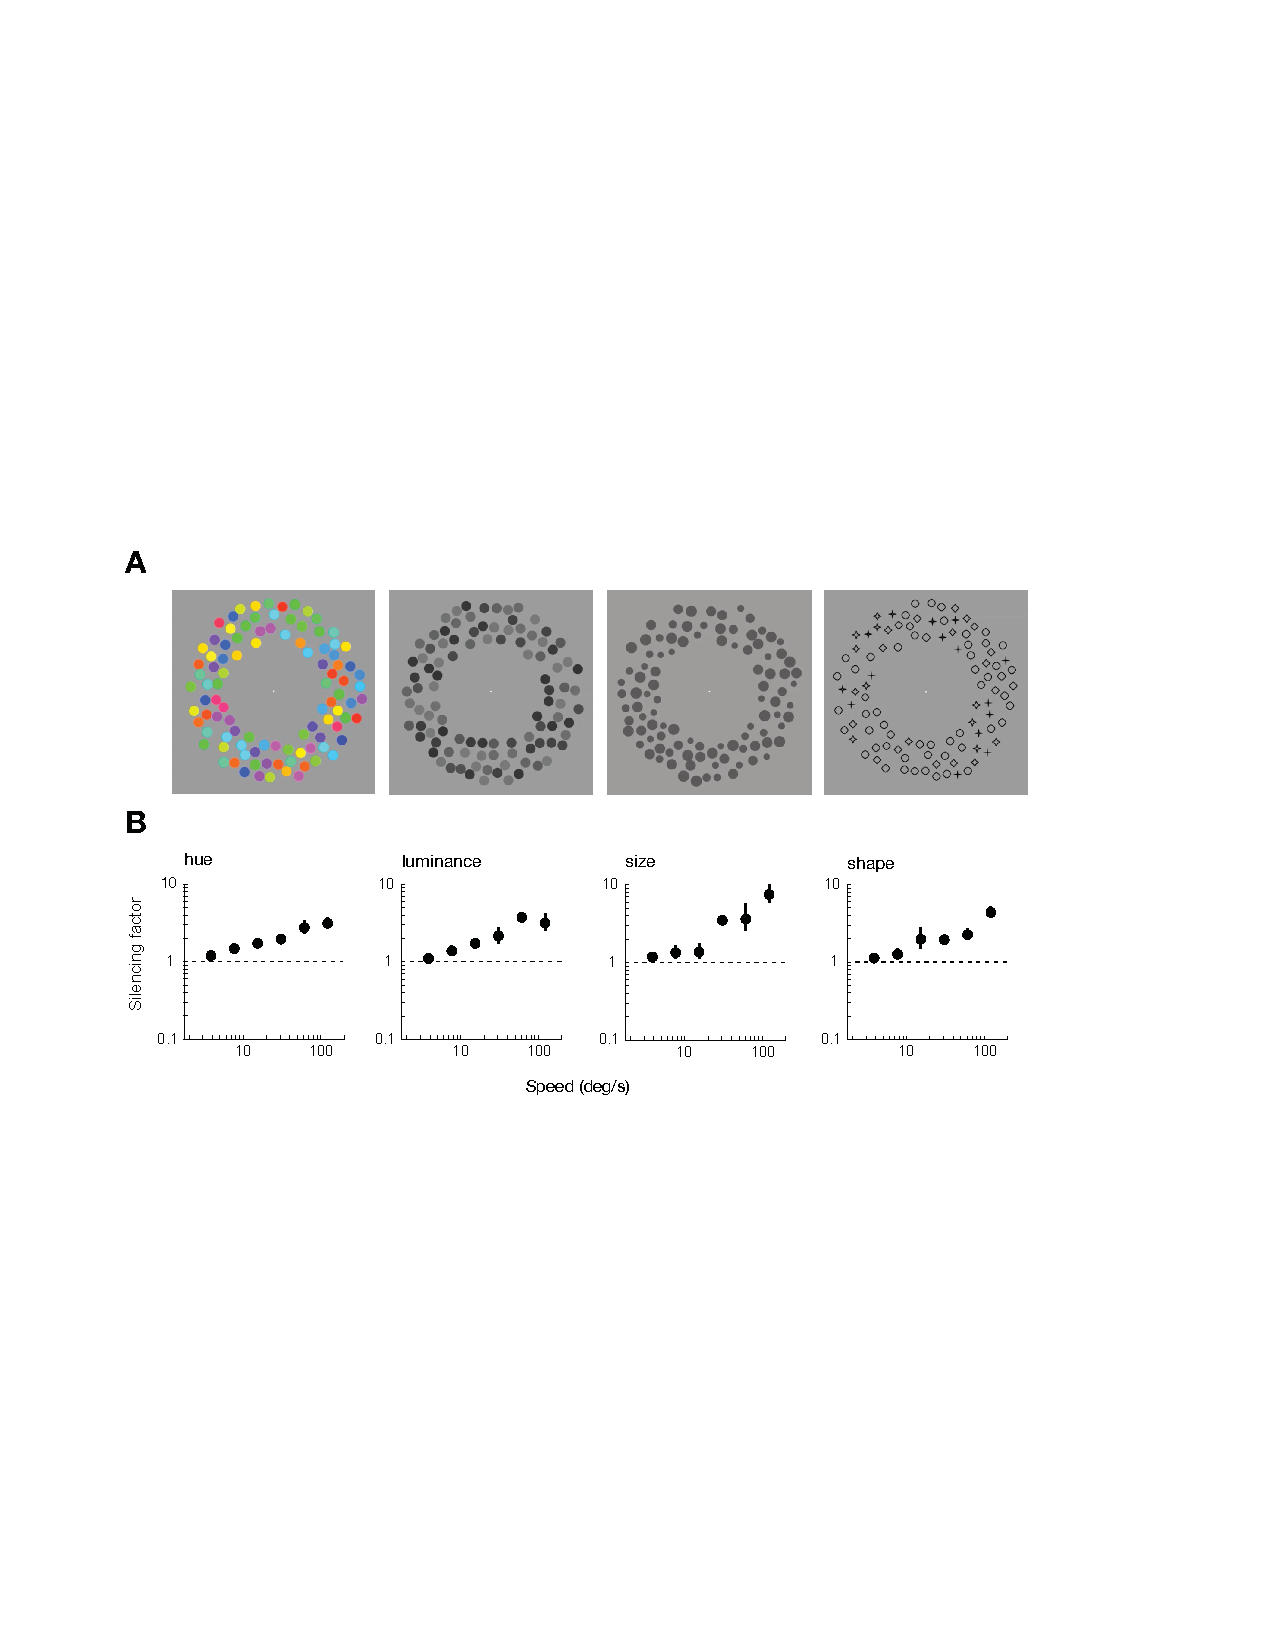
\includegraphics[width=\textwidth]{figures/fig1}
%\caption[Short figure name.]{This is a figure that floats inline and here is its caption.
%\label{fig:myInlineFigure}}
%\end{figure}

%% Requires fltpage2 package
%%
% \begin{FPfigure}
% 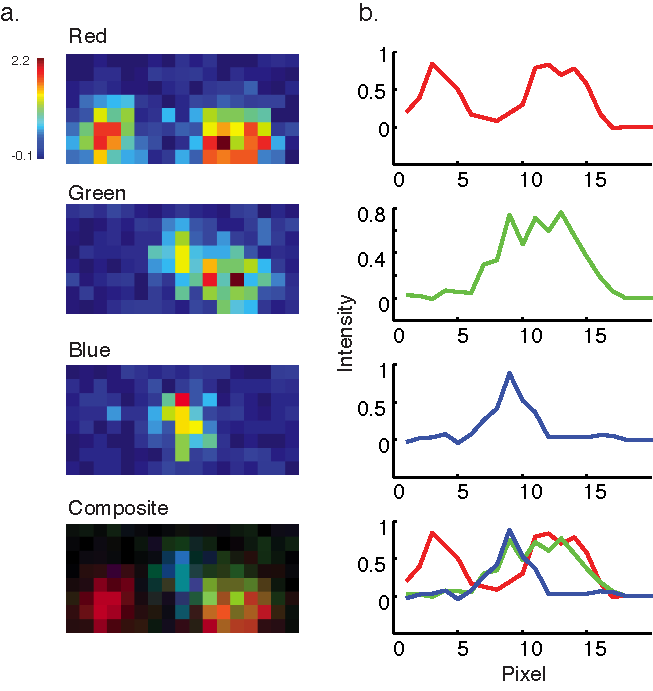
\includegraphics[width=\textwidth]{figures/fullpage}
% \caption[Short figure name.]{This is a full page figure using the FPfigure command. It takes up the whole page and the caption appears on the preceding page. Its useful for large figures. Harvard's rules about full page figures are tricky, but you don't have to worry about it because we took care of it for you. For example, the full figure is supposed to have a title in the same style as the caption but without the actual caption. The caption is supposed to appear alone on the preceding page with no other text. You do't have to worry about any of that. We have modified the fltpage package to make it work. This is a lengthy caption and it clearly would not fit on the same page as the figure. Note that you should only use the FPfigure command in instances where the figure really is too large. If the figure is small enough to fit by the caption than it does not produce the desired effect. Good luck with your thesis. I have to keep writing this to make the caption really long. LaTex is a lot of fun. You will enjoy working with it. Good luck on your post doctoral life! I am looking forward to mine. \label{fig:myFullPageFigure}}
% \end{FPfigure}
% \afterpage{\clearpage}


